\documentclass[11pt]{article}
\usepackage{amsmath, amsfonts, amsthm, amssymb}  % Some math symbols
\usepackage{enumerate}
\usepackage{fullpage}
\usepackage{color}
\usepackage[x11names, rgb]{xcolor}
\usepackage{tikz}
\usepackage{graphicx}
\usepackage{listings}
\usepackage{fancyhdr}
\usepackage{pdflscape}
\usepackage{hyperref}

\lstset{basicstyle=\ttfamily, 
        breaklines=true,
        columns=fullflexible, 
        numbers=left, 
        numbersep=10pt, 
        numberstyle=\sffamily\footnotesize\color{gray}}

% \usepackage{fontspec}
% \setmainfont{Times New Roman}

\renewcommand*{\familydefault}{\sfdefault}

\setlength{\parindent}{0pt}
\setlength{\parskip}{6pt}
\pagestyle{empty}

\pagestyle{fancy}
\fancypagestyle{firststyle}
{
   \lhead{\myname \\ \myandrew \\ \today \\ \vspace*{-.5em}}
   \rhead{15-221 \\ Fall 2014 \\ Section A \\ \vspace*{-.5em}}
   \setlength{\headsep}{50pt}
}

\newcommand{\myname}{Justin Gallagher, Ted Li}
\newcommand{\myandrew}{jgallagher@cmu.edu, wenxuanl@andrew.cmu.edu}
\newcommand{\mytitle}{Instructions}
\title{Creating a Simple Chrome Extension\\ \vspace*{.5em} \Large\mytitle}
\date{}
%%%%%%%%%%%%%%%%%%%%%%%%%%%%%%%%%%%%%%%%%%%%%%%%%%%%%%%%%%%

\begin{document}

\pagenumbering{gobble} 
\author{~\\
\normalsize {\bf Submitted to}\\
\normalsize Thomas M. Keating\\
\normalsize Assistant Teaching Professor\\
\normalsize School of Computer Science\\
\normalsize Carnegie Mellon University\vspace*{2em}\\
\normalsize {\bf Prepared by}\\
\normalsize Justin Gallagher\\
\normalsize Ted Li\vspace*{2em}\\
\normalsize School of Computer Science\\
\normalsize Carnegie Mellon University\\
\normalsize \today}

\clearpage\maketitle
\thispagestyle{firststyle}

\newpage
\lhead{\myname}
\rhead{\thepage}
\setlength{\headsep}{25pt}
\tableofcontents
\newpage
\pagenumbering{arabic} 
\setlength{\voffset}{-50pt}
\setlength{\headsep}{25pt}

\section{Overview}

\subsection{Introduction}

Chrome extensions allow you to add features and functionality to Google's Chrome browser without modifying source code. This guide will walk you through creating a simple extension and uploading it to the Chrome Web Store for the public to download.

The tutorial has 5 steps and can be completed in approximately 15 minutes.

\subsection{Motivation}

Chrome extensions allow you to add features and functionality to Google's Chrome browser without modifying source code. The framework utilizes web development technologies such as HTML, CSS, and JavaScript which may already be familiar to you. Extensions are also modular, so you can build many which work in their own environments without conflict. Finally, Chrome extensions can be easily distributed to users through the Chrome Web Store, allowing wide adoption of your creations.

\subsection{Requirements}

For this guide, you will need:

\begin{enumerate}
	\item A Internet connected Windows / Mac computer with Google Chrome installed.
	\item A text editor in which you are proficient.
	\item A Google account.
	\item \$5 to pay Google's developer registration fee.
	\item A simple logo for your Chrome extension.
	\item Elementary skills in HTML and JavaScript.
\end{enumerate}

\subsection{Goal}

By the end of this guide, you will have created a simple Chrome extension which produces a pop-up window reading "Hello world!" when a button in the top right toolbar is clicked. The extension will also be available for the general public to download onto their browser from the Chrome Web Store.

\subsection{Cautions and Warnings}

An incorrectly written extension can cause undesired behavior resulting in an unstable browser. Uploading such an extension can cause it to be removed from the Chrome Web Store and your developer account to be banned. Remember to test your extension thoroughly before uploading!

\newpage

\section{Understanding the Constituents of a Google Chrome Extension}

This section covers the basic constituents that are required for any Google Chrome extension. Usually, Chrome extensions are packaged as a zipped archive of a folder. The archive consists of all the resources that a Chrome extension requires to run its functionalities. The files in the archive may include images, web pages or source code that the extension will find useful.

\section{Creating a Chrome Extension}
\subsection{Step 1: Create a Folder For Our Project}

For this tutorial, we will be putting everything related to our extension under the \texttt{My Chrome Extension} folder on the Desktop. As the first step, create a new folder on the Desktop named \texttt{My Chrome Extension}.

	\begin{figure}[htb]
	\centering
	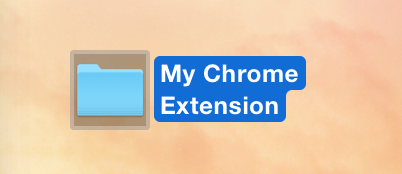
\includegraphics[width=.3\textwidth]{figures/folder.png}
	\caption{Creating the folder on the Desktop\label{fig:folder}}
	\end{figure}

\subsection{Step 2: Declaring the Manifest File}

After creating a folder for our project, we'll need to create a manifest file named \texttt{manifest.json}. A manifest file can be viewed as a configuration file for any Chrome Extension that configures specific settings of our Chrome extension, such as icon, version number, extension name and description. At a high level, we'll use the manifest file to declare to Chrome its functionalities, and what permissions it requires in order to complete these functions.

For this tutorial, we will name our Chrome extension `My Chrome extension', and we will also designate an icon for our Chrome extension. Feel free to replace the name, icon and description with your own.

Open up any text editor and save the following code snippet to the folder we just created, and name the file \texttt{manifest.json}.

\begin{lstlisting}[mathescape]
{
  "manifest_version": 2,
  "name": "My Chrome extension",  // The name for our Chrome extension
  "description": "This is a simple extension intended as a demonstration!",
  "version": "1.0",  // The current version for our Chrome extension
  "browser_action": { "default_icon": "icon.png", "default_popup": "popup.html" }
}
\end{lstlisting}

After this step, our folder should look like this:

	\begin{figure}[htb]
	\centering
	\vspace*{-2em}
	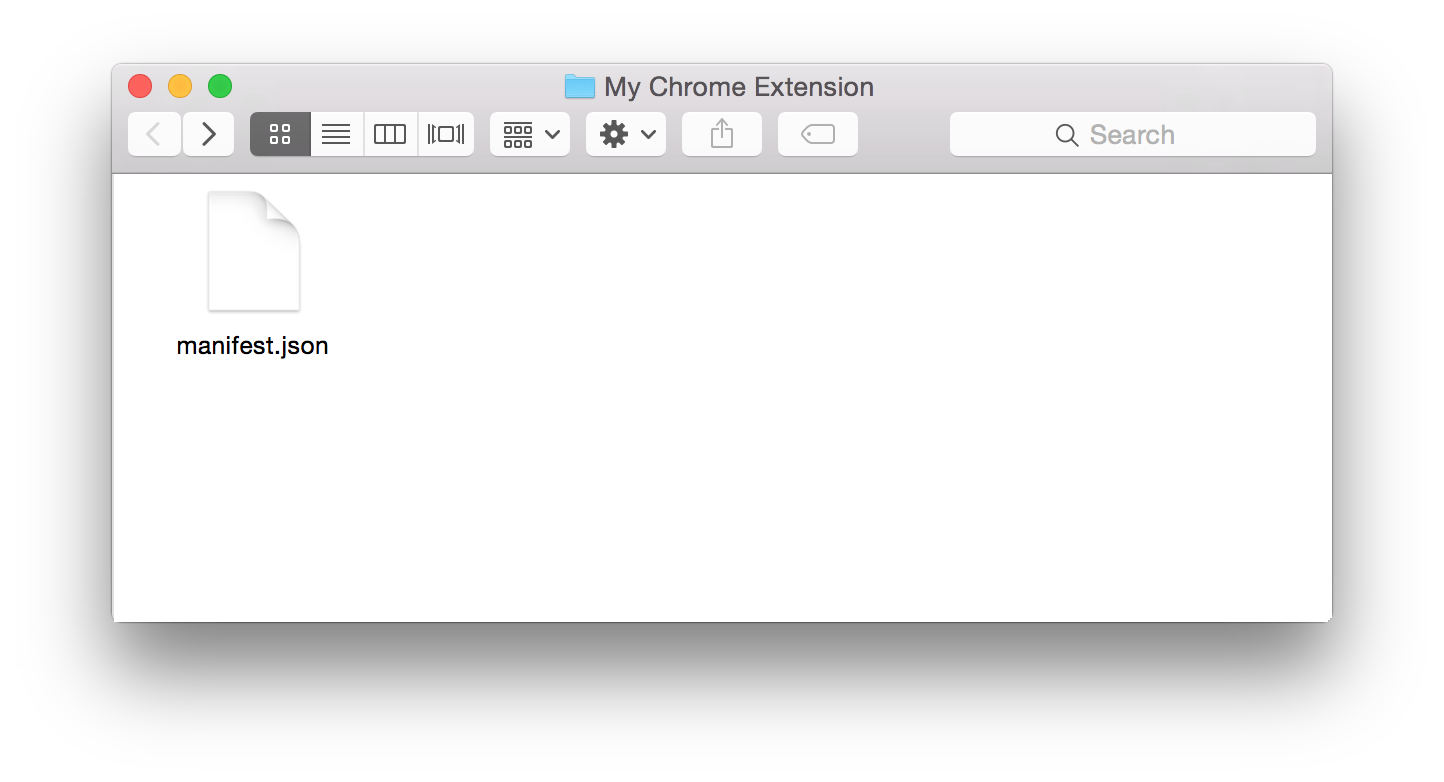
\includegraphics[width=\textwidth]{figures/manifest.png}\vspace*{-2em}
	\hspace*{-2.5em}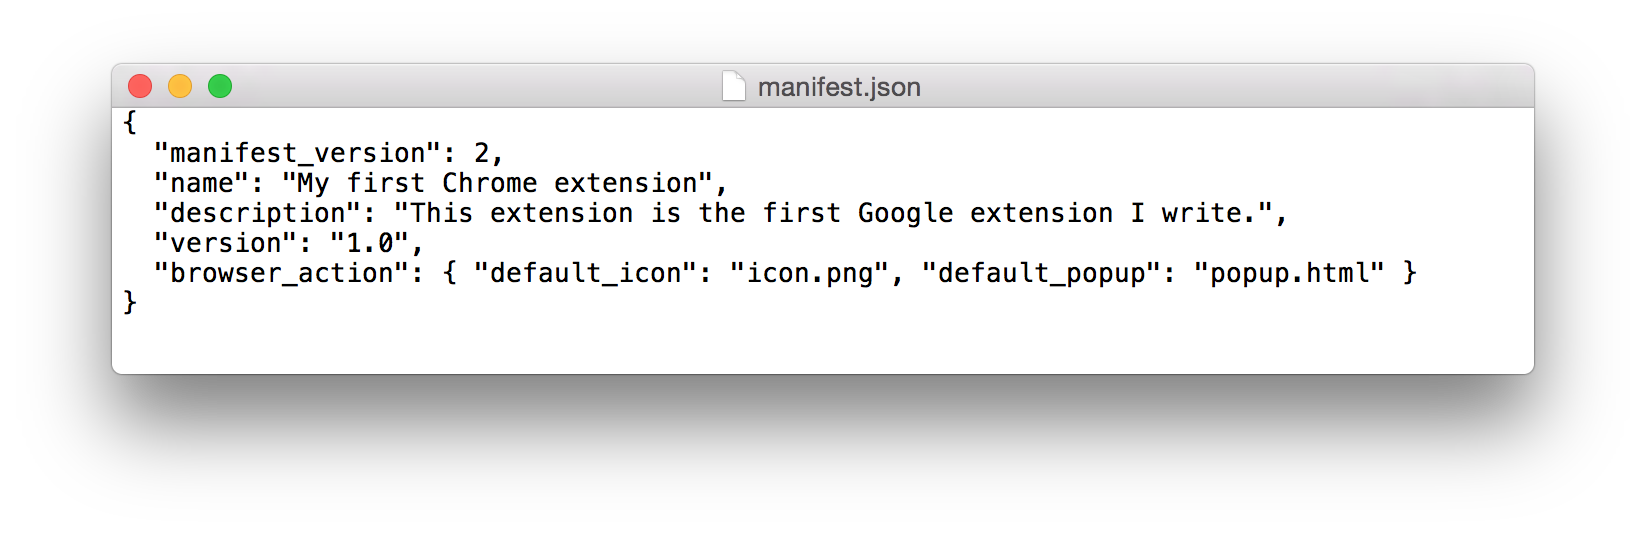
\includegraphics[width=1.1\textwidth]{figures/saving.png}
	\vspace*{-2em}
	\caption{Creating the \texttt{manifest.json} file\label{fig:saving}}
	\vspace*{1em}
	\end{figure}

\subsection{Step 3: Adding In the Resources For the Chrome Extension}

By now, you probably have noticed that there were two files in the \texttt{manifest.json} file that we haven't yet created. Now, we should proceed to create the two resource files. They are called resource files because they are files that Google Chrome will eventually use to render our extension to users.

For this tutorial, we will be using the following icon. You may choose any icon you like.

	\begin{figure}[htb]
	\centering
	
\includegraphics[width=.1\textwidth]{figures/icon128.png}
	\end{figure}

Save the icon into the folder named \texttt{icon.png}. 

Next, create a file in the same folder named \texttt{popup.html} with the following content:
\begin{lstlisting}[mathescape]
<!doctype html>
<html>
  <head>
    <title>Hello World!</title>
  </head>
  <body>
  Hello World!
  </body>
</html>
\end{lstlisting}

Our folder should now look like this:

	\begin{figure}[htb]
	\centering
	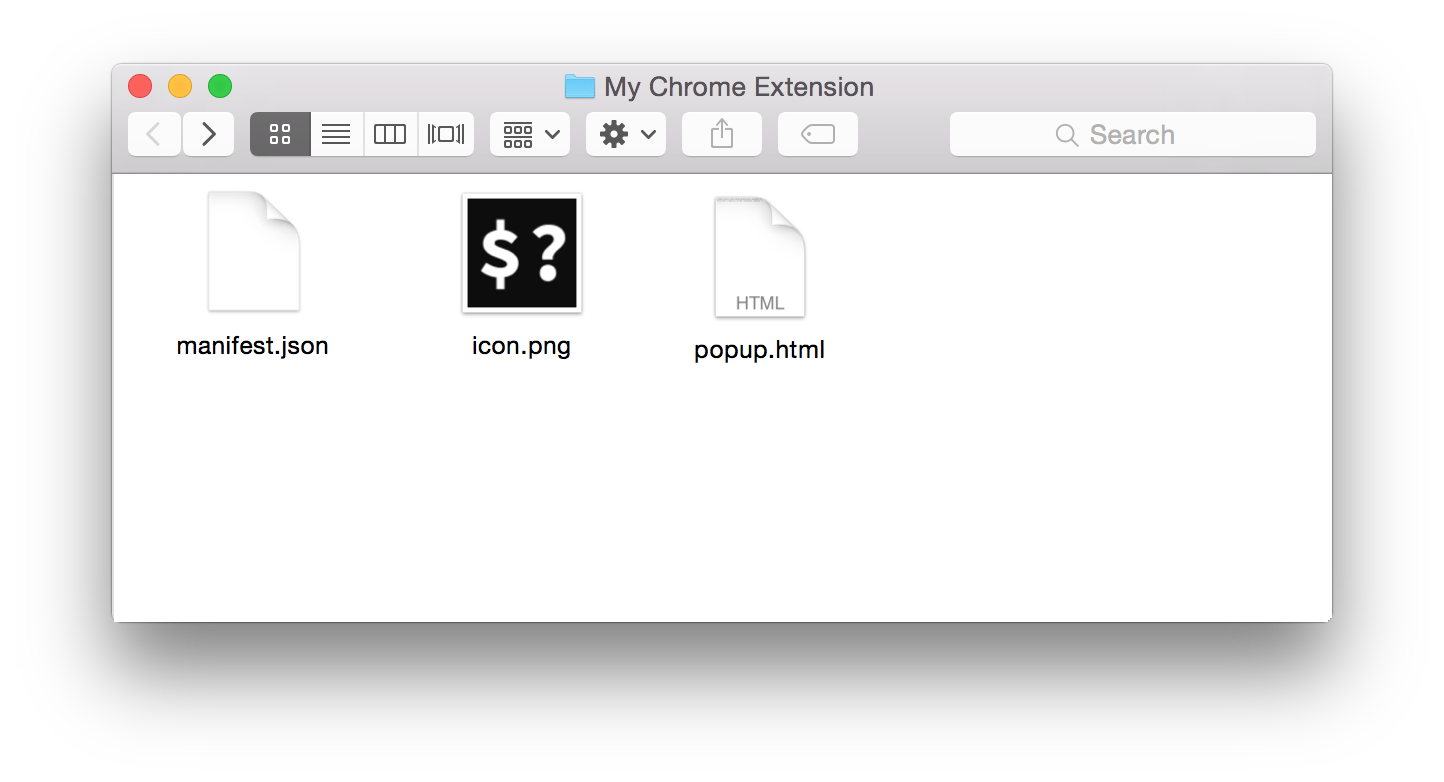
\includegraphics[width=\textwidth]{figures/all.png}
	\vspace*{-2.5em}
	\caption{Adding the resource files\label{fig:all}}
	\end{figure}

Now that we have created the extension, let's import into the Google Chrome browser and give it a try!

\section{Adding the Extension to Chrome}

This step outlines how to add the extension you wrote to your installation of Chrome, and how to run the application for yourself.

\begin{enumerate}
	\item Open your Google Chrome browser and visit \texttt{chrome://extensions}.
	\item At the top right of the page, ensure that the ``Developer Mode'' checkbox is checked, as shown in \emph{Figure \ref{fig:devmode}}. If it is not, click the box next to the text label to activate Developer Mode.

	\begin{figure}[htb]
	\centering
	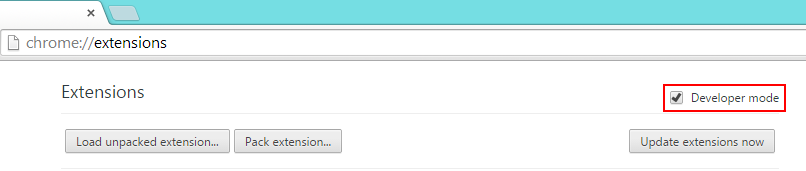
\includegraphics[width=1\textwidth]{figures/devmode.png}
	\caption{Enabling Chrome developer mode\label{fig:devmode}}
	\end{figure}

	\item Press the ``Load unpacked extension...'' button and select the folder containing your \texttt{manifest.json} file, as shown in \emph{Figure \ref{fig:loadext}}. Press ``OK'' to load your extension.

	\begin{figure}[htb]
	\centering
	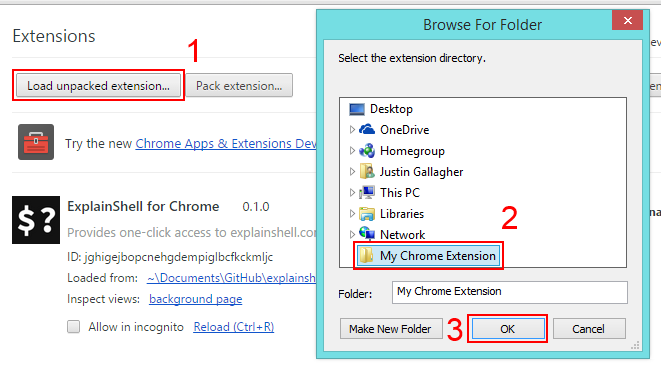
\includegraphics[height=0.5\textwidth]{figures/loadext.png}
	\caption{Adding your extension to Chrome\label{fig:loadext}}
	\end{figure}

	\item When your extension is properly loaded, you should see an entry for ``My Chrome Extension'' in the extensions list, as shown in \emph{Figure \ref{fig:loadedext}}.

	\begin{figure}[htb]
	\centering
	\vspace*{-1em}
	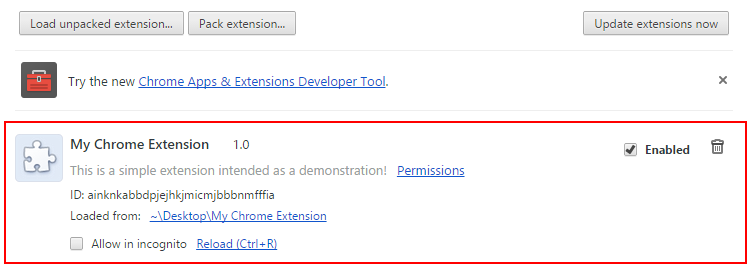
\includegraphics[width=.9\textwidth]{figures/loadedext.png}
	\caption{A successfully loaded extension\label{fig:loadedext}}
	\vspace*{-1em}
	\end{figure}
\end{enumerate}

\newpage
Now your extension has been loaded into the browser, and you should immediately see the extension you have written take effect.

Simply open up a new browser window, and you should already see the icon of our extension available on the toolbar. If you click the icon, a small popup will appear that says ``Hello World!'', as shown in \emph{Figure \ref{fig:ext}}.

	\begin{figure}[htb]
	\centering
	\vspace*{-1em}
	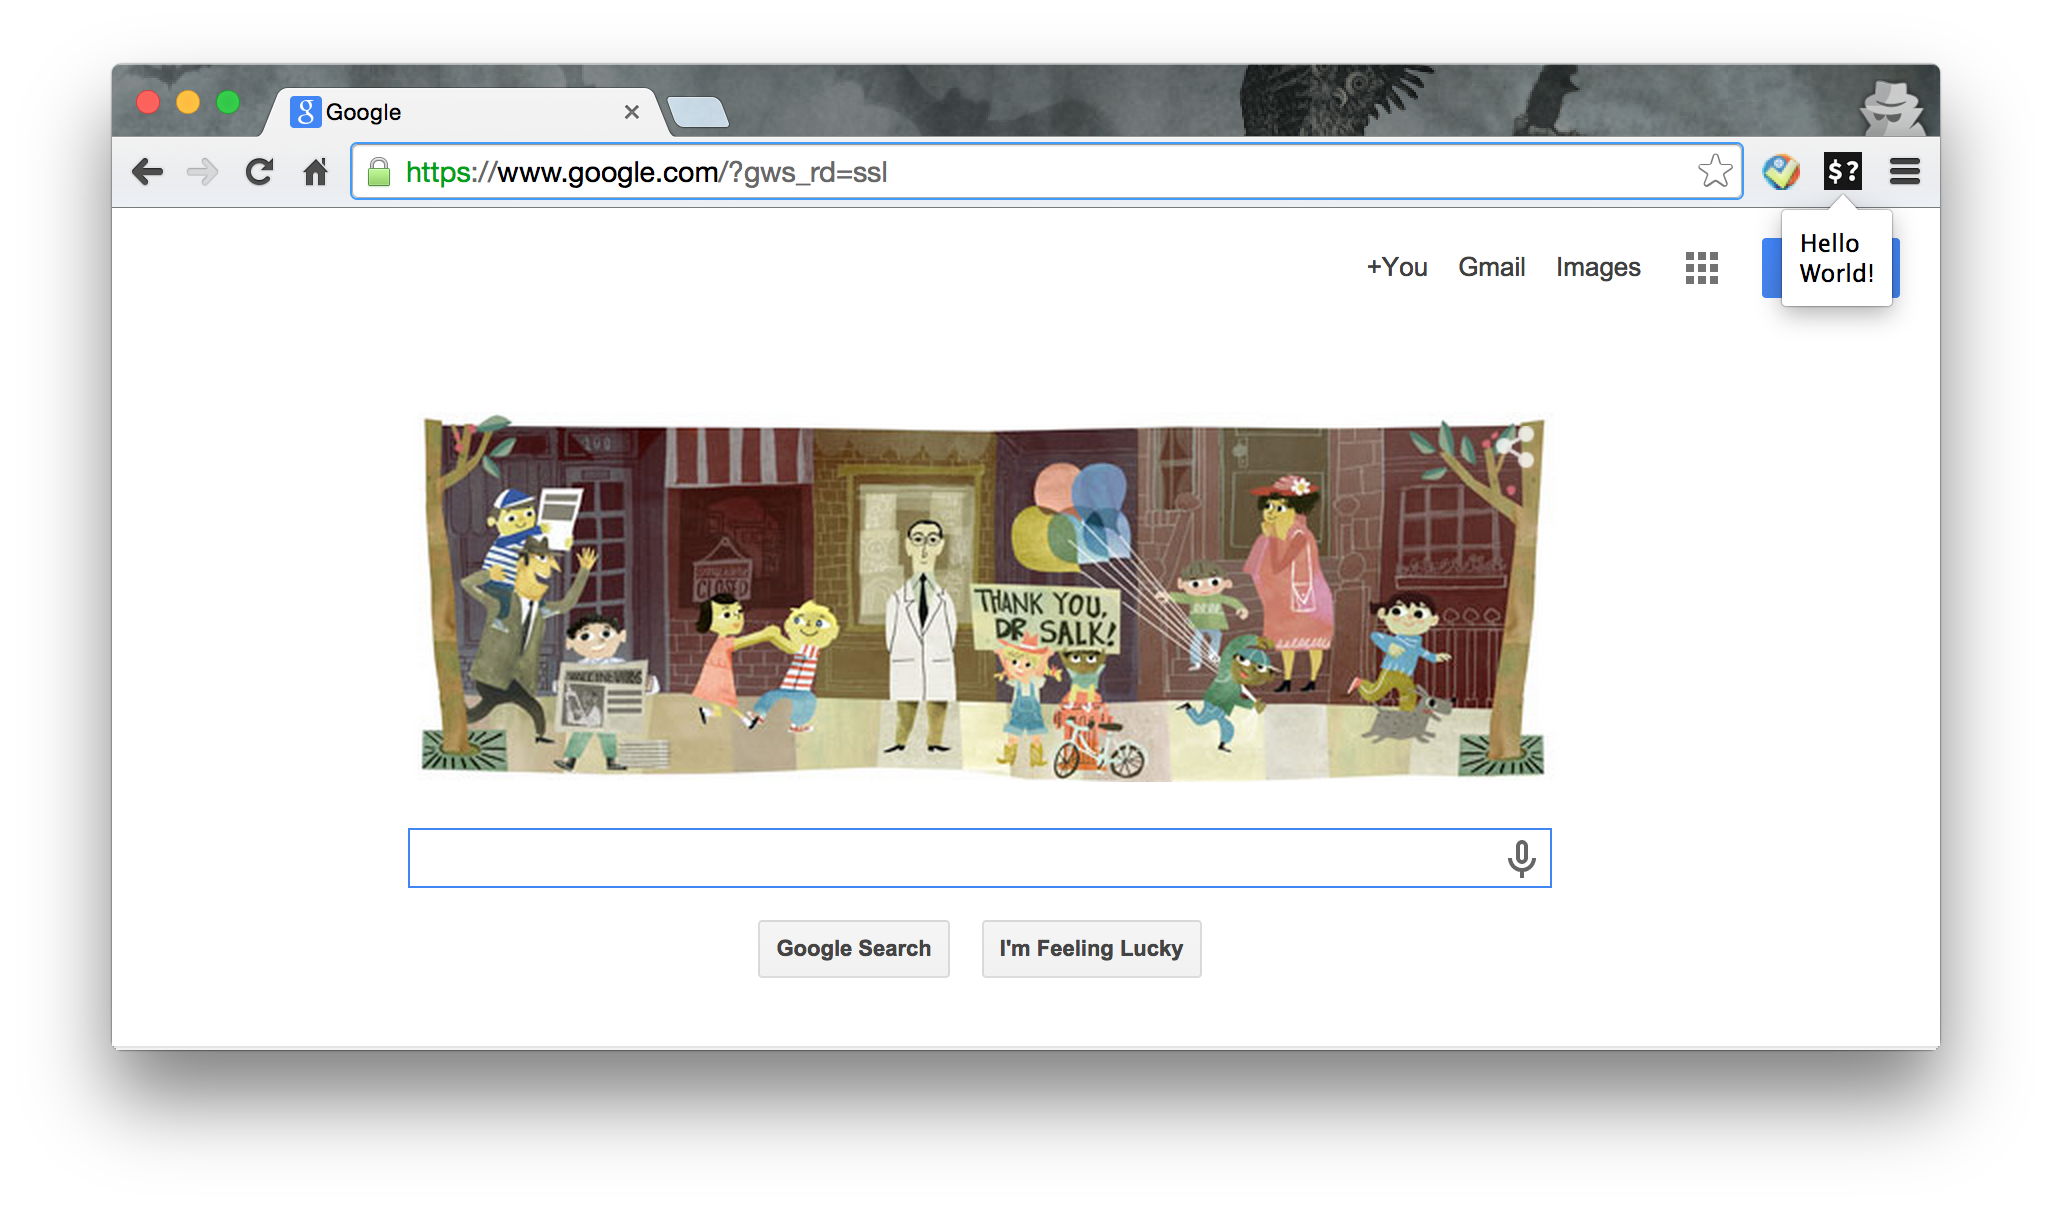
\includegraphics[width=1\textwidth]{figures/ext.png}
	\vspace*{-1em}
	\caption{Our Chrome Extension in Action\label{fig:ext}}
	\end{figure}

Proceed to the next step to learn how to upload your extension to the Chrome Web Store for others to download.

\section{Uploading the Extension to the Chrome Web Store}

This step shows you how to upload your app to the Chrome Web Store for others to download and use.

\begin{enumerate}
	\item Zip your extension directory. To do this in Windows, open Windows Explorer, right click on the directory, and choose ``Send to'', then click ``Compressed (zipped) folder'', as shown in \emph{Figure \ref{fig:zipext}}.\\

	\begin{figure}[htb]
	\centering
	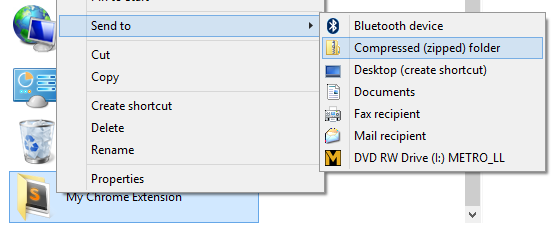
\includegraphics[width=0.7\textwidth]{figures/zipext.png}
	\caption{Zipping a directory in Windows Explorer\label{fig:zipext}}
	\end{figure}

	\item Navigate to the Chrome Web Store Developer Dashboard at \\\texttt{https://chrome.google.com/webstore/developer/dashboard}, and sign in to your Google Account.

	\item If this is your first time publishing an application through Google, you will need to pay Google's \$5 registration fee. A yellow banner will be displayed on the dashboard if you need to pay this fee, as in \emph{Figure \ref{fig:regfee}} - press the ``Pay this fee now'' button and follow Google's instructions to enable your developer account.\\

	\begin{figure}[htb]
	\centering
	
\includegraphics[width=1\textwidth]{figures/regfee.png}
	\caption{Google developer registration fee notice\label{fig:regfee}}
	\end{figure}

	\item Click the ``Add New Item'' button on the dashboard. Here, you will be prompted to upload your extension's \texttt{.zip} file, created in substep 1. Click ``Choose file'', and select the \texttt{.zip} file, as shown in \emph{Figure \ref{fig:uploadext}}. Press the ``Upload'' button to complete the transaction.\\

	\begin{figure}[htb]
	\centering
	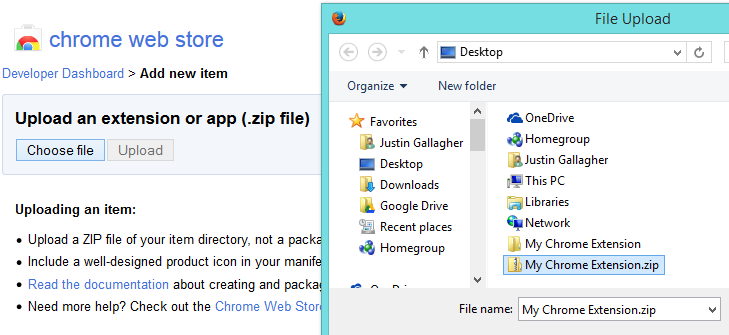
\includegraphics[width=0.7\textwidth]{figures/uploadext.png}
	\caption{Uploading your extension to Google\label{fig:uploadext}}
	\end{figure}

	\item You will now be redirected to a page where you can configure the store appearance of your extension. There are many options available on this page, but most are optional. Make sure you set the ``Category'' and ``Language'' fields of the form to appropriate values. Click ``Publish changes'' to publish your app to the Chrome store. It may take up to an hour for your extension to appear to others. When you are done, your extension will have a page in the Web Store as in \emph{Figure \ref{fig:publishedext}}.\\

	\begin{figure}[htb]
	\centering
	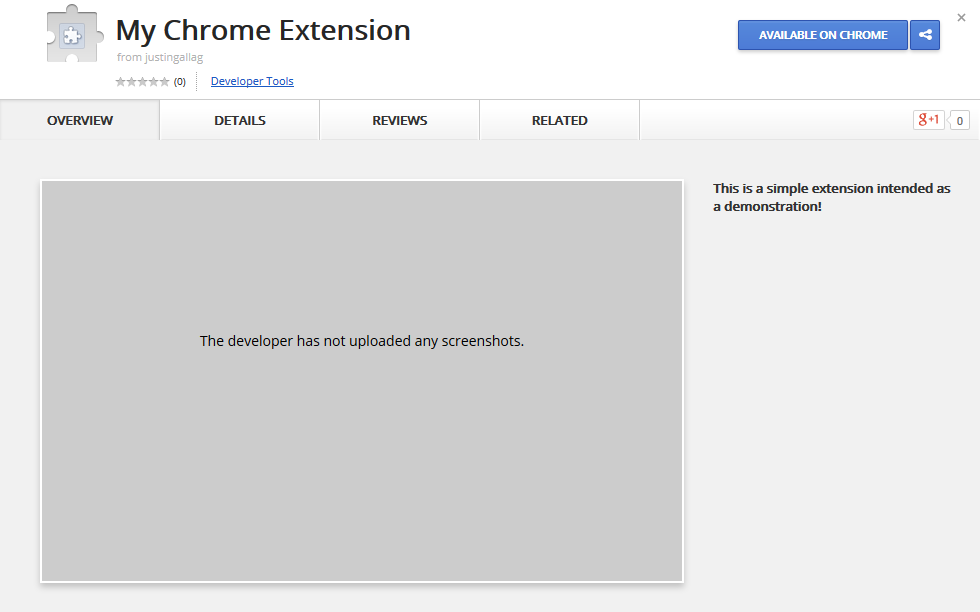
\includegraphics[width=0.7\textwidth]{figures/publishedext.png}
	\caption{Store page for a completed extension\label{fig:publishedext}}
	\end{figure}
\end{enumerate}

Your extension will now be available for public download, and can be found in the Chrome Web Store's search.
\end{document}
